\documentclass[tikz,border=3pt]{standalone}
\usepackage[utf8]{inputenc}
\usepackage[T1]{fontenc}
\usepackage{libertinus}
\usepackage{amsmath,amssymb}
\usepackage{pgfplots}
\pgfplotsset{compat=1.18}
\usetikzlibrary{arrows.meta}
\definecolor{UGblue}{RGB}{0,51,102}
\begin{document}
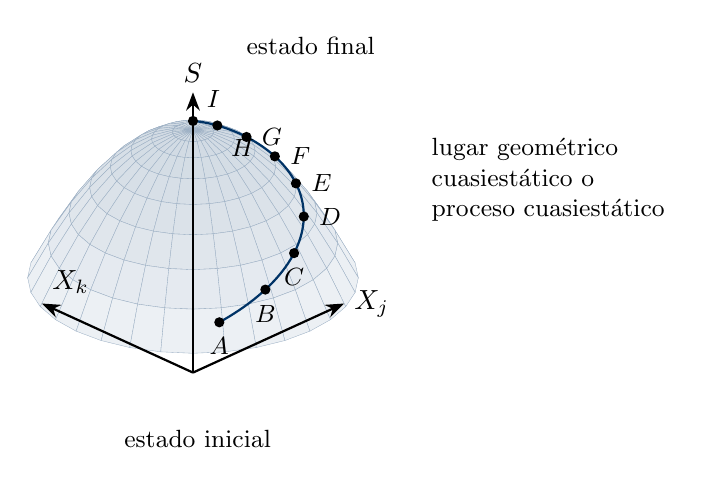
\begin{tikzpicture}
\begin{axis}[hide axis,view={-45}{34},width=9.5cm,height=9cm,xmin=-1.6,xmax=1.6,ymin=-1.6,ymax=1.6,zmin=0,zmax=1.6,z buffer=sort,clip=false,>=Stealth,
  colormap={s}{color(0cm)=(UGblue!6) color(1cm)=(UGblue!18)}]
\addplot3[surf,shader=flat,draw=UGblue!40,line width=0.12pt,domain=0:1.2,y domain=0:360,samples=9,samples y=33,z buffer=sort]
  ({x*cos(y)},{x*sin(y)},{1.3-0.55*x*x});
\draw[->,thick] (axis cs:0,0,0) -- (axis cs:1.55,0,0) node[right] {$X_j$};
\draw[->,thick] (axis cs:0,0,0) -- (axis cs:0,1.55,0) node[above right] {$X_k$};
\draw[->,thick] (axis cs:0,0,0) -- (axis cs:0,0,1.5) node[above] {$S$};
\draw[thick,UGblue] plot[domain=0:1,samples=80,variable=\t] (axis cs:{(1.1-0.7*\t)*cos(235+170*\t)},{(1.1-0.7*\t)*sin(235+170*\t)},{1.3-0.55*(1.1-0.7*\t)^2});
\node[font=\small,anchor=west] at (axis cs:0.75,0.3,1.5) {estado final};
\node[font=\small,anchor=east] at (axis cs:-0.5,-1.4,0.1) {estado inicial};
\node[font=\small,align=left,anchor=west] at (axis cs:1.45,-0.9,0.9) {lugar geométrico\\cuasiestático o\\proceso cuasiestático};
\node[circle,fill,inner sep=1.3pt,label={[font=\small]below:$A$}] at (axis cs:-0.6309,-0.9011,0.6345) {};
\node[circle,fill,inner sep=1.3pt,label={[font=\small]below:$B$}] at (axis cs:-0.2407,-0.9835,0.7362) {};
\node[circle,fill,inner sep=1.3pt,label={[font=\small]below:$C$}] at (axis cs:0.1207,-0.9171,0.8294) {};
\node[circle,fill,inner sep=1.3pt,label={[font=\small]right:$D$}] at (axis cs:0.4028,-0.7343,0.9142) {};
\node[circle,fill,inner sep=1.3pt,label={[font=\small]right:$E$}] at (axis cs:0.5745,-0.4821,0.9906) {};
\node[circle,fill,inner sep=1.3pt,label={[font=\small]right:$F$}] at (axis cs:0.6273,-0.2130,1.0586) {};
\node[circle,fill,inner sep=1.3pt,label={[font=\small]right:$G$}] at (axis cs:0.5745,0.0251,1.1182) {};
\node[circle,fill,inner sep=1.3pt,label={[font=\small]below right:$H$}] at (axis cs:0.4462,0.1963,1.1693) {};
\node[circle,fill,inner sep=1.3pt,label={[font=\small]above right:$I$}] at (axis cs:0.2828,0.2828,1.2120) {};
\end{axis}
\end{tikzpicture}
\end{document}
